\chapter[Rivelazione di muoni cosmici]{Rivelazione di muoni cosmici con SiPM e scintillatore}\label{cap3}
\section{I muoni}
Un muone, indicato con il simbolo $\mu^-$, è una particella elementare, cioè una particella subatomica che non è composta da altre particelle. Secondo il modello standard,
i muoni appartengono alla famiglia dei fermioni, cioè delle particelle che hanno spin semintero. All'interno della famiglia dei fermioni,
i muoni appartengono al gruppo dei leptoni, sono cioè dei fermioni elementari. Queste caratteristiche sono condivise anche dall'elettrone,
con la differenza che i muoni sono 207 volte più pesanti \cite{officeofscience_doe}. Essendo così pesanti, i muoni subiscono un'accelerazione meno intensa dai campi
elettromagnetici, risultando estremamente penetranti nella materia; trovandone traccia anche dentro le miniere.

Come si può osservare dalla \autoref*{fig:muoncascade}, i muoni si formano naturalmente negli strati più alti dell'atmosfera a seguito del
decadimento di altri tipi di particelle, chiamate pioni. Questi si formano quando i raggi cosmici, che sono formati da protoni con energie
elevatissime, collidono con i nuclei atomici delle molecole che si trovano in aria.
I muoni, dopo la loro formazione, iniziano a muoversi nello spazio a velocità prossime a quelle della luce, fino ad arrivare sulla superficie
terrestre. I muoni hanno tempo di decadimento a riposo pari a \SI{2}{\micro\second}, tempo che, secondo la fisica classica, non gli
permetterebbe di raggiungere la superficie terrestre \cite{muonsources_about}. Tuttavia, muovendosi a velocità vicine a quelle della luce, secondo la teoria della
relatività, il loro tempo di vita risulta dilatato rispetto a chi, nello stesso sistema inerziale, rimane fermo; allo stesso modo, collocandoci
nel sistema di riferimento del muone, in accordo con la legge di contrazione delle lunghezze, la particella vede la distanza contratta.
\begin{figure}[h!]
    \centering
    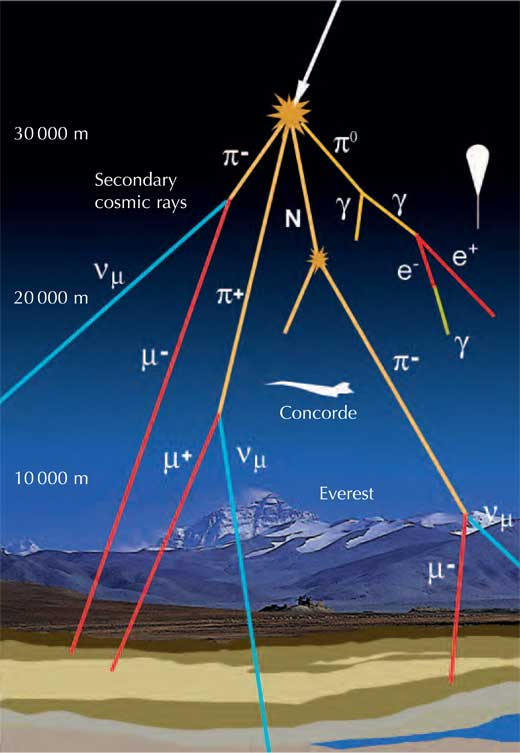
\includegraphics[width=.65\linewidth]{img/muoncascade.jpg}
    \caption{Il processo di formazione dei muoni \cite{luu_2020_decode}.}
    \label{fig:muoncascade}
\end{figure}

Come gli elettroni, anche i muoni sono particelle dotate di carica negativa $-e$, questo li porta ad avere energia sufficiente per
ionizzare le molecole. Questo tipo di energia è detta radiazione ionizzante. I muoni sono la radiazione ionizzante più penetrante.
\section{Descrizione del setup di misura}
Nel~\autoref*{caratterizzazione_sipm} è stato descritto il processo di caratterizzazione del SiPM, grazie al quale è stato possibile
stabilire i corretti parametri di funzionamento del dispositivo. In questo capitolo, si descrive l'esperimento effettuato in laboratorio
attraverso il quale è stato possibile utilizzare in combinazione dei SiPM con uno scintillatore. Quest'ultimo è un materiale
in cui la ionizzazione prodotta dalla radiazione incidente induce l'emissione di luce. Il processo di rivelazione funziona come segue: il muone
incidente deposita energia tramite la radiazione ionizzante quando incontra lo scintillatore \cite{yang_2022_mugrid} \cite{leoni_2021_scintillator}. La radiazione ionizzante è composta da particelle
subatomiche o onde elettromagnetiche che hanno sufficiente energia per ionizzare atomi o molecole. Nel caso dello scintillatore, l'energia
depositata dalla radiazione ionizzante libera fotoni. Se uno scintillatore è usato in combinazione con un rilevatore di luce, come un SiPM, è
possibile creare un sistema che operi come rilevatore del passaggio di particelle ionizzanti.

Questa configurazione è quella usata nel caso preso in esame per la rivelazione di muoni cosmici. Per ottimizzare la resa della rivelazione, si collocano i SiPM il più
vicino possibile allo scintillatore, anche adiacenti se la conformazione dei due oggetti lo permette. Per poter funzionare, il setup, ha
bisogno di essere polarizzato, bisogna cioè fornire la tensione di alimentazione. Avendo collegato due SiPM e lo scintillatore, abbiamo
bisogno di una tensione di alimentazione sufficientemente elevata, di circa \SI{42}{\volt}. Per fornire questa tensione è stato utilizzato,
ancora una volta il DC Power Analyzer Keysight N6705C. Anche in questo caso, per preservare i componenti, si alza
gradualmente la tensione di \SI{1}{\volt} al secondo, a partire da \SI{0} fino a \SI{43}{\volt}. Inoltre, per evitare che il SiPM rilevi
radiazioni luminose non provenienti dallo scintillatore, lo si pone in un ambiente buio. Nel caso preso in cosiderazione in questo lavoro,
durante le acquisizioni lo scintillatore era posto in un ambiente completamente buio avvolto da un materiale oscurante, all'interno di una scatola.

Completato l'allestimento del setup, il sistema è pronto per rilevare eventuali muoni in arrivo. Si stima che, sulla superficie terrestre, ogni
minuto arrivi un muone per \si{\square\centi\meter}. Quando un muone arriva, è previsto un cambiamento dell'andamento della tensione in uscita
dal sistema. Per poter osservare l'andamento della tensione nel tempo in un punto di un circuito si usa uno strumento chiamato oscilloscopio.
Questo strumento è dotato di un display che consente di visualizzare, su un grafico, l'andamento nel dominio del tempo della tensione presente
nel nodo del circuito a cui è collegato l'oscilloscopio.
Nel caso preso in esame, è stato utilizzato l'oscilloscopio LeCroy WaveSurfer 454. Questo oscilloscopio digitale, permette anche di salvare
i grafici ottenuti ed è dotato del sistema operativo Windows XP Embedded. Queste ultime due caratteristiche rendono possibile il salvataggio
delle forme d'onda su un dispositivo di archiviazione che può essere poi collegato ad un comune calcolatore per effettuare l'analisi dei dati.

Il SiPM e l'oscilloscopio sono sempre collegati tra di loro rendendo continuo il rilevamento delle tensioni in uscita.
Per evitare quindi il salvataggio continuo di dati, è necessario stabilire in quale condizione salvare i dati ricevuti.
Dopo vari tentativi, è stato scelto di salvare i grafici quando veniva rilevato un valore di tensione, detto trigger, pari a \SI{-50}{\milli\volt}.
Questo valore permette di avere un numero di eventi acquisiti comparabile al numero di muoni in arrivo sulla terra.

Nella \autoref*{fig:setup_rivelazione_muoni} è mostrato il setup completo utilizzato nella rivelazione dei muoni cosmici.

Per alimentare il circuito e leggere il valore di tensione in uscita al SiPM si utilizza il circuito mostrato nella \autoref*{fig:circuito_lettura_alimentazione}.
Al canale per la lettura del segnale proveniente dal SiPM va collegato un connettore a T. Nella \autoref*{fig:setup_rivelazione_muoni}, si
può vedere che al connettore a T sono collegati l'oscilloscopio e i due SiPM. In questo modo, l'oscilloscopio salverà i dati quando, su almeno
uno dei due lati dello scintillatore su cui sono montati i SiPM sarà erogata una tensione sufficiente da far scattare il trigger. Il sistema
funziona in modo simile ad una porta OR: è sufficiente che uno dei due SiPM eroghi una tensione minima pari a quella del trigger per fare in
modo che l'oscilloscopio salvi i dati ottenuti. La decisione di usare il connettore a T è stata presa in quanto l'interesse del lavoro è misurare
il passaggio del muone e di valutare le prestazioni dello scintillatore e del SiPM in confronto alle simulazioni e alla caratterizzazione.

\begin{figure}[h!]
    \centering
    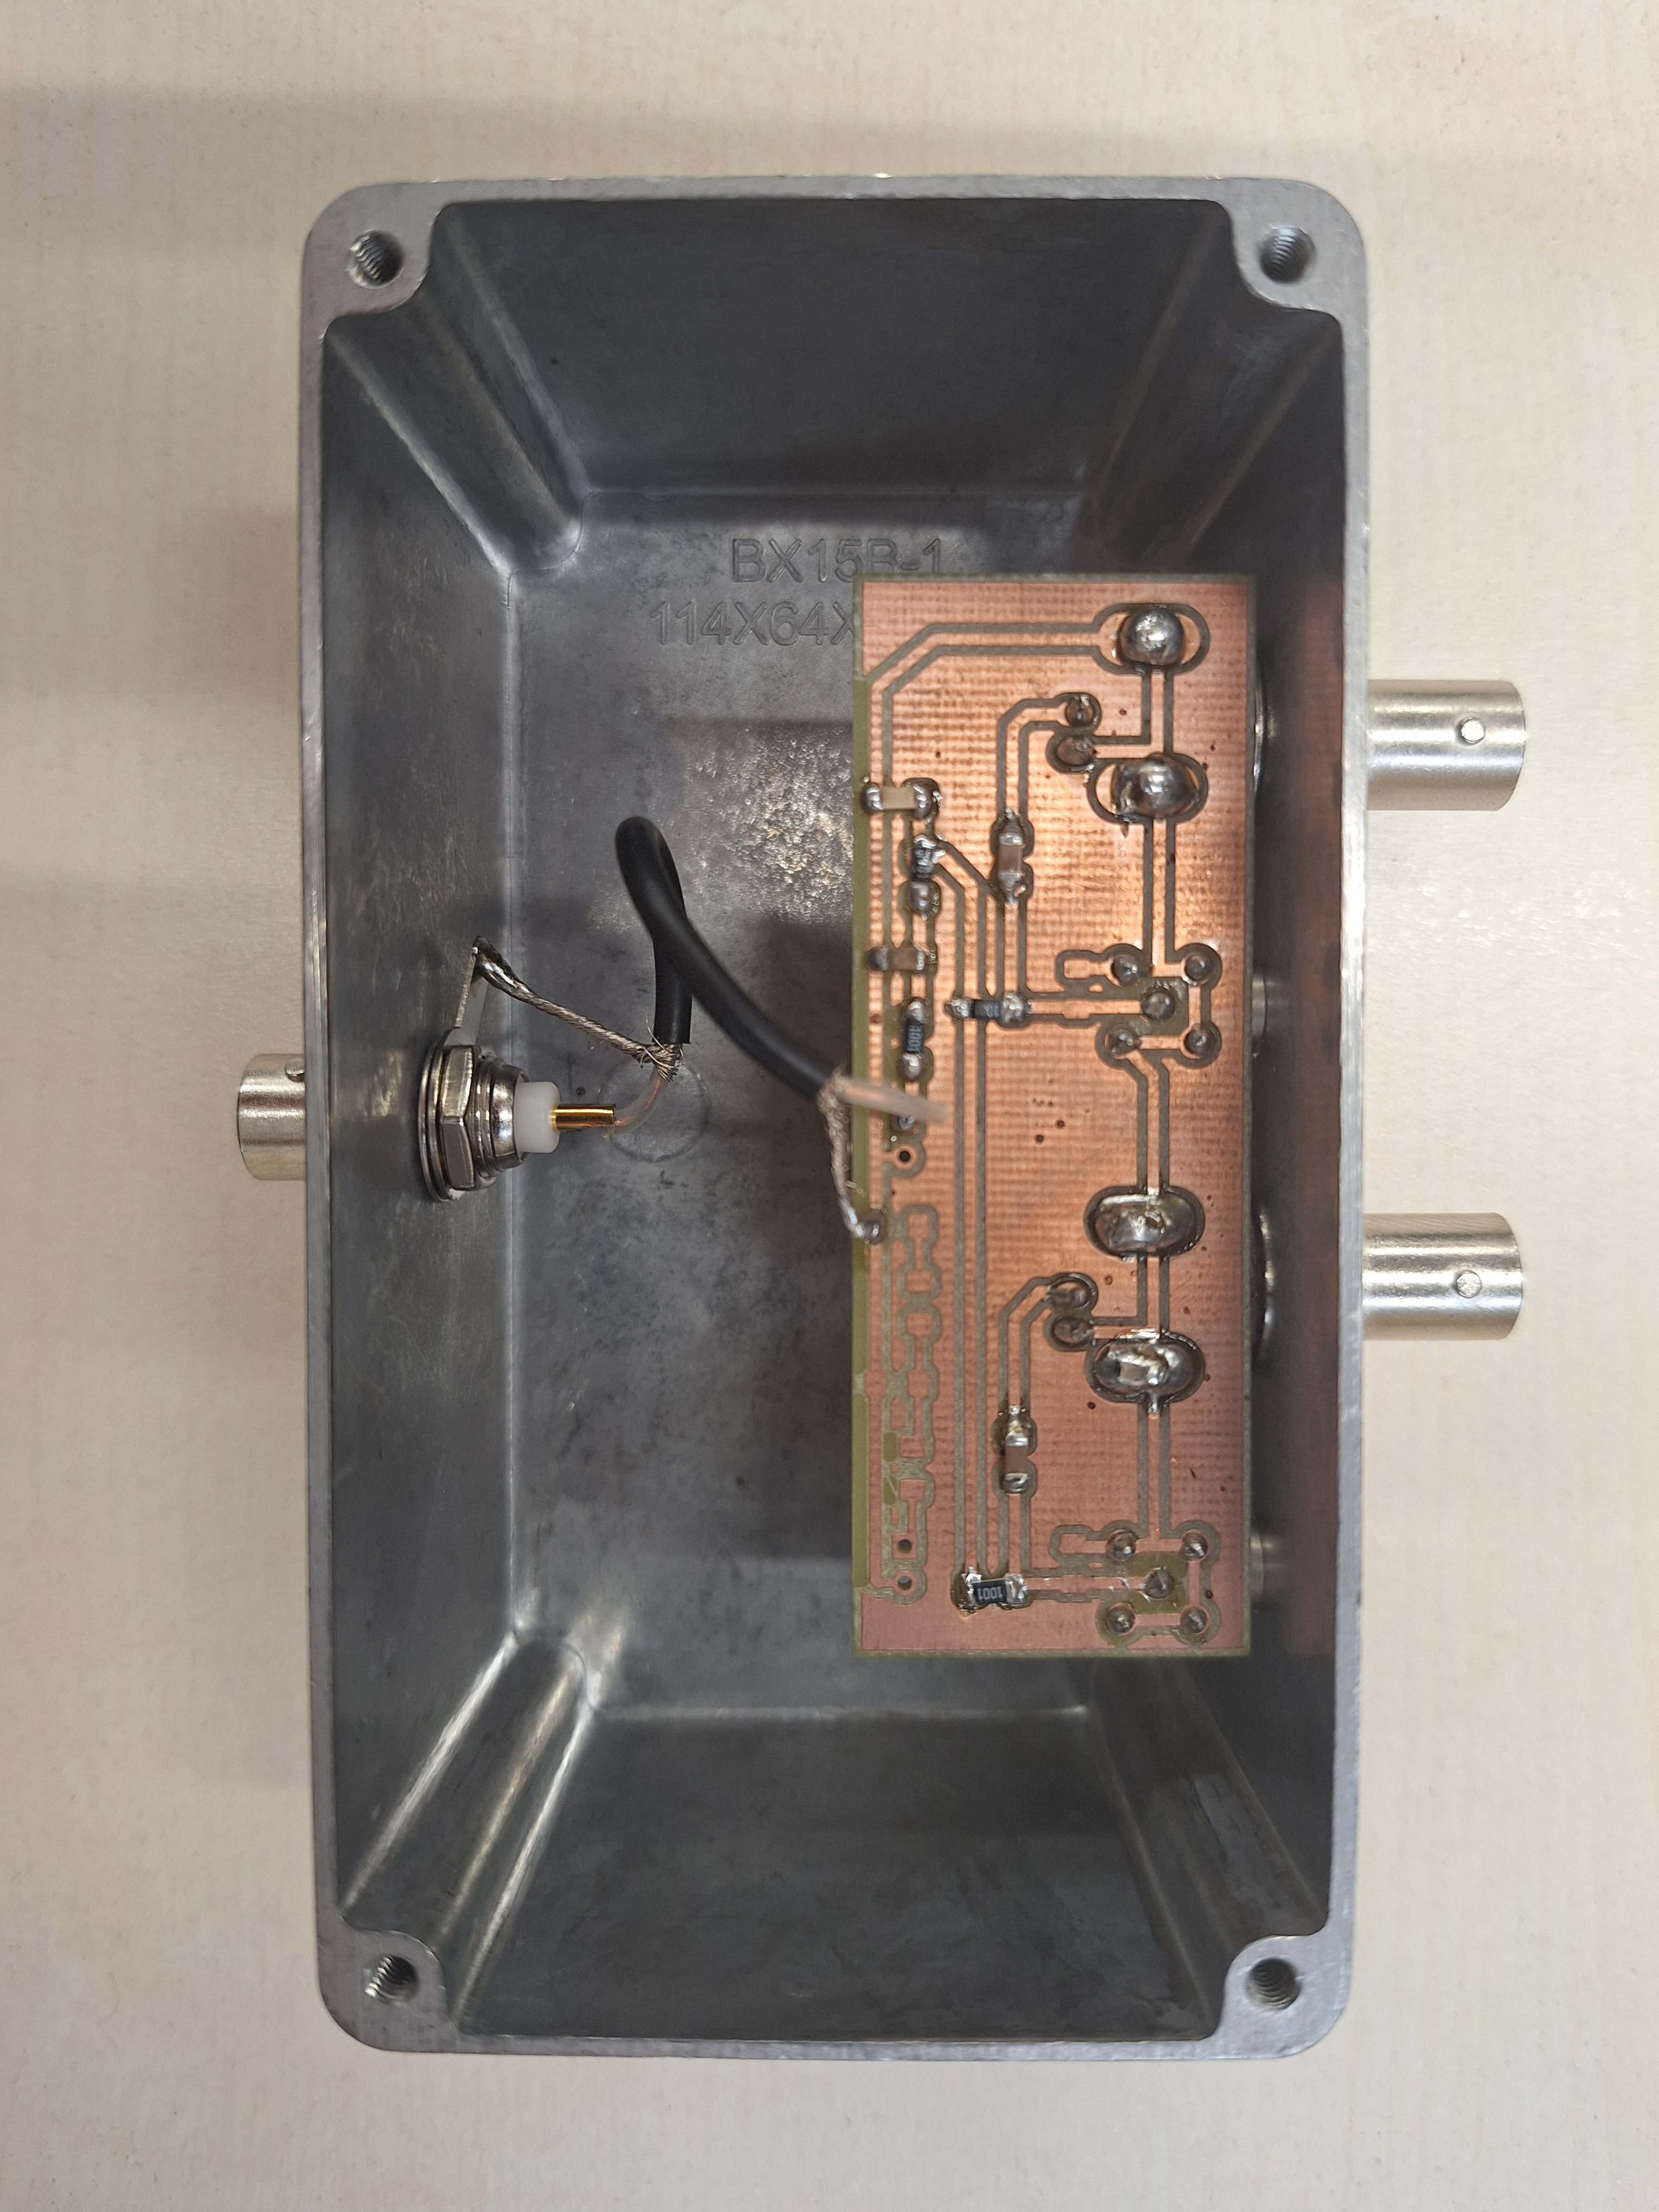
\includegraphics[width=.75\linewidth]{img/circuito_lettura_alimentazione.jpg}
    \caption{Il circuito utilizzato per l'alimentazione e per la lettura del segnale in uscita dal SiPM. Sono presenti tre connettori:
        quella a sinistra è per l'alimentazione, i due di destra sono usati per la lettura del segnale. Nel caso analizzato è stato utilizzato
        solo uno dei due connettori di lettura.}
    \label{fig:circuito_lettura_alimentazione}
\end{figure}

\begin{figure}[h!]
    \centering
    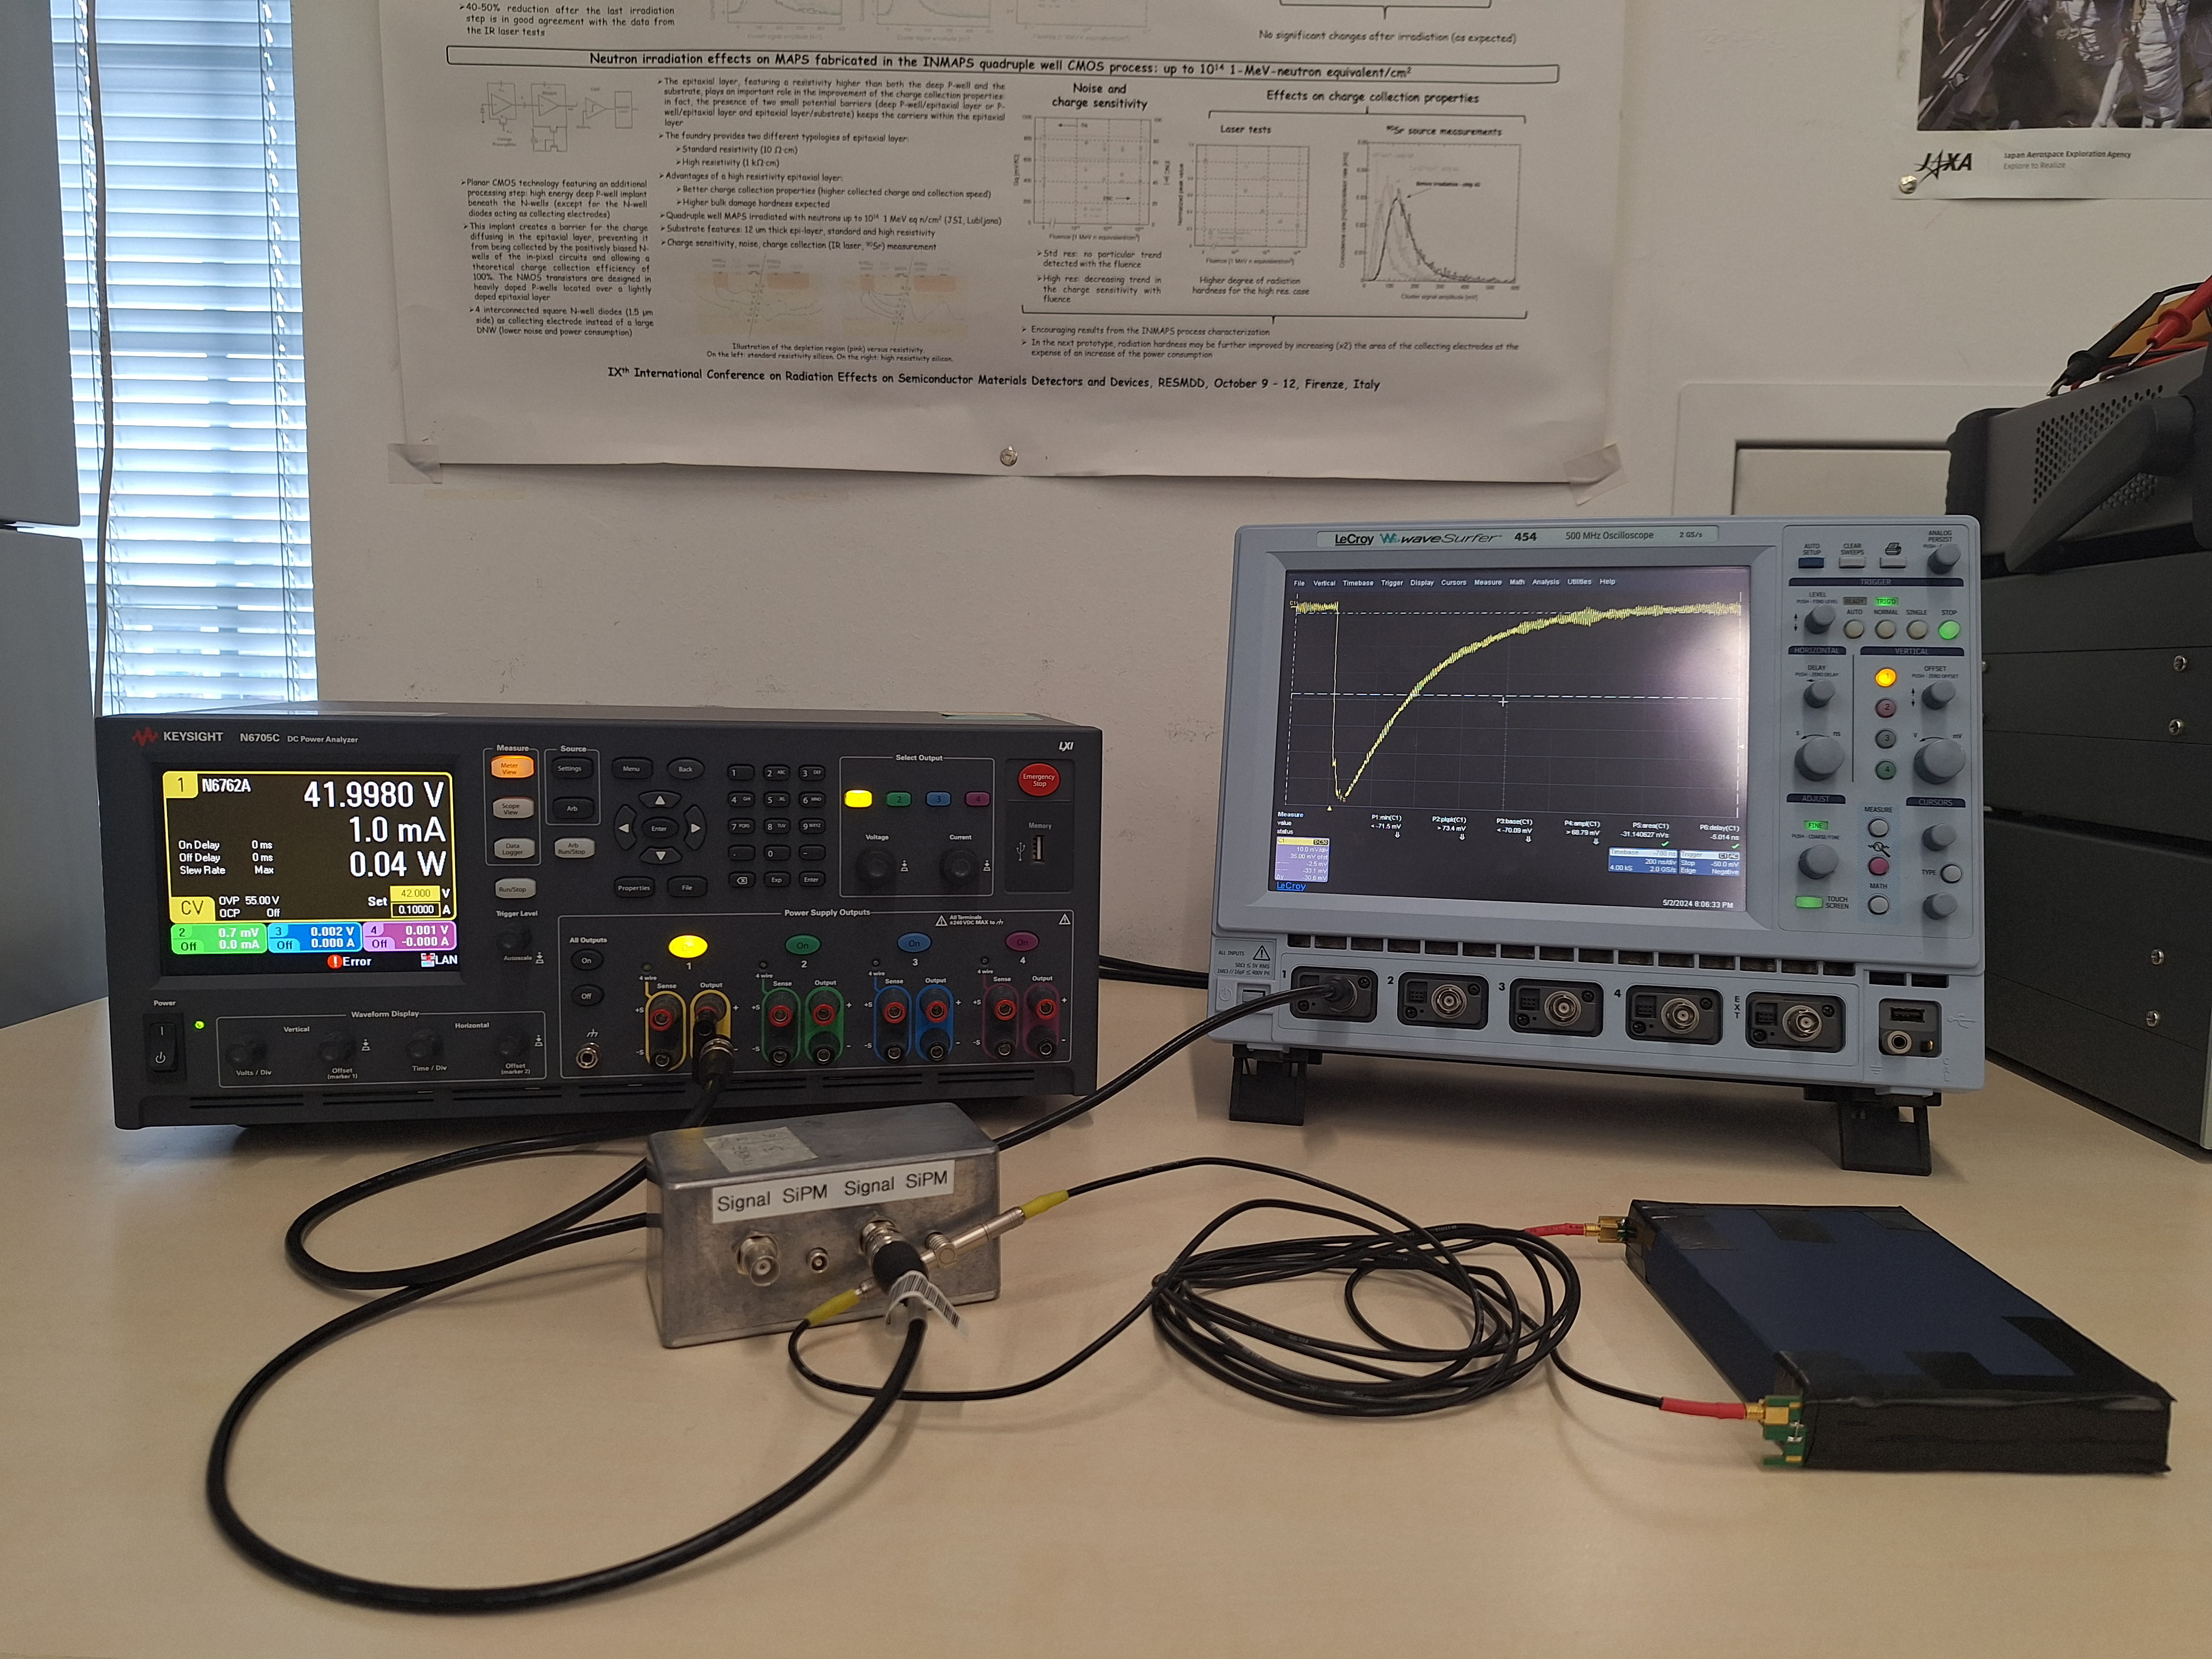
\includegraphics[width=.75\linewidth]{img/setup_rilevazione_muoni.jpg}
    \caption{Il setup usato per la rivelazione dei muoni cosmici. A sinistra il DC Power Analyzer, in alto a destra l'oscilloscopio e in basso a
        destra lo scintillatore con i due SiPM. Lo scintillatore e i due SiPM sono circondati da un involucro per minimizzare le radiazioni luminose e
        non che possono colpirli.}
    \label{fig:setup_rivelazione_muoni}
\end{figure}

\section{Raccolta e analisi dei dati}
Dopo aver predisposto il setup, è possibile rilevare l'arrivo di muoni sullo scintillatore. Questo è segnalato da un cambiamento della
tensione in uscita dal SiPM, e si può notare sul display dove appare un'immagine simile a quella della \autoref*{fig:oscilloscopio_display}.
\begin{figure}[h!]
    \centering
    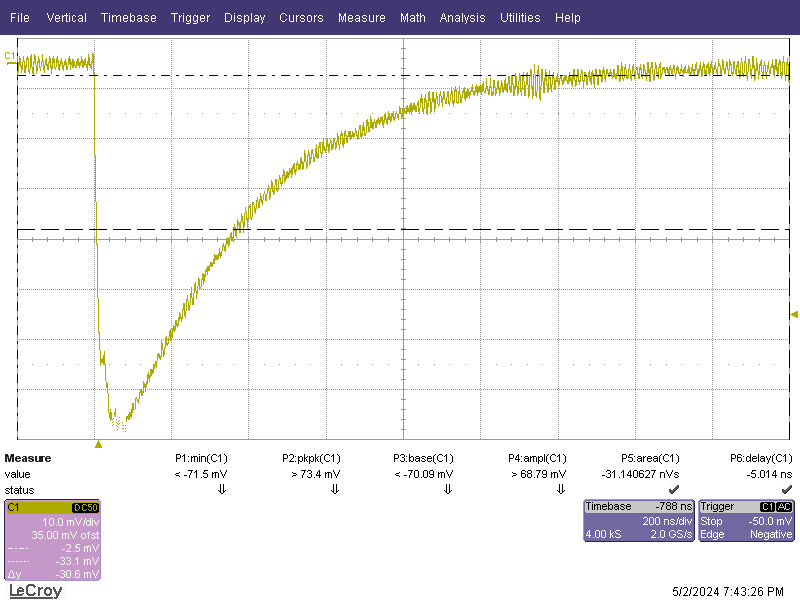
\includegraphics[width=.75\linewidth]{img/oscilloscopio_display.png}
    \caption{Il display dell'oscilloscopio che mostra l'andamento della tensione di uscita del SiPM all'arrivo di un muone.}
    \label{fig:oscilloscopio_display}
\end{figure}

Una volta raggiunto il trigger, l'oscilloscopio salva sul dispositivo di archiviazione i valori di tensione misurati in un determinato
istante di tempo. In questo modo è possibile, una volta spostati i file sul calcolatore, elaborare i dati ottenuti. Usando Python, in
particolare l'interfaccia \texttt{Pyplot} presente nella liberia \texttt{Matplotlib} possiamo realizzare il grafico che otteniamo
sull'interfaccia del display. Un esempio di grafico ottenuto in questo modo è quello in \autoref*{fig:20240502_single_bias_42V_trig_m50mV_box_indoor}.
\begin{figure}[h!]
    \centering
    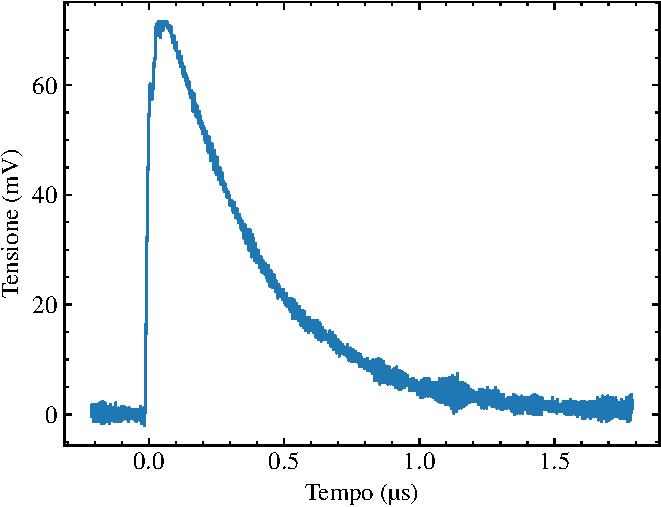
\includegraphics[width=.75\linewidth]{img/20240502_single_bias_42V_trig_m50mV_box_indoor.pdf}
    \caption{Grafico ottenuto a partire dai dati raccolti dall'oscilloscopio che mostra l'andamento della tensione di uscita del SiPM all'arrivo di un muone.
        In questo caso il grafico è stato trasformato nel suo simmetrico rispetto all'asse delle ascisse per avere una maggiore leggibilità.}
    \label{fig:20240502_single_bias_42V_trig_m50mV_box_indoor}
\end{figure}
Come possibile apprezzare, vengono salvati i valori a partire da circa \SI{200}{\nano\second} prima dell'arrivo del trigger fino a circa
\SI{2}{\micro\second} dopo l'arrivo del trigger. La finestra temporale è stata impostata sull'oscilloscopio, ed è stata determinata in forma
empirica per garantire di valutare l'intero andamento del segnale fino al ritorno al valore di tensione che si ha nel punto DC.

Osservando il grafico, si notano parecchie oscillazioni dovute al rumore esterno soprattutto nei momenti in cui si è in attesa dell'arrivo
del muone e subito dopo il suo arrivo durante il ritorno in fase di riposo. Questo aspetto è rilevante nel momento in cui le variazioni
della baseline causate dal rumore, potrebbero erroneamente triggerare il salvataggio dei dati e, nel caso di raccolta dati più massiccia,
lasciando acceso il sistema per qualche minuto, si ottiene un quantitativo di dati tale da poter avere delle misure non volute. Includere
queste misure nell'analisi, potrebbe portare a conclusioni errate. È necessario, quindi, scartare queste ipotetiche forme molto
rumorose. Per farlo si possono usare vari metodi. Uno di questi può essere quello di scartare le misure che hanno un numero
estremamente elevato di oscillazioni. Tuttavia, applicare questo metodo ai grafici ottenuti può portare a scartare delle misure che hanno
numerose oscillazioni prima o dopo il trigger, anche se questo è dovuto al passaggio del muone. Questo problema può essere risolto
filtrando le oscillazioni con frequenza più elevata. Lo strumento che permette di fare ciò
è un filtro passa-basso. Il subpackage \texttt{signal} del modulo \texttt{scipy} fornisce varie funzioni con cui realizzare dei filtri
passa-basso. Il più comune e semplice di questi è il filtro Butterworth. La funzione di trasferimento per questa classe di filtri è definita
dalla \autoref*{eq:filtro_Butterworth}. In questa equazione, $n$ è detto ordine del filtro e $\omega_f$ è la pulsazione di taglio, cioè la
pulsazione che si ha in corrispondenza di un guadagno di \SI{-3}{\dB}.
\begin{equation}
    \left | G(j \omega) \right | = {\frac{1}{\sqrt{ 1 + \left ( \frac{\omega}{\omega_f} \right ) ^ {2 n}} } }
    \label{eq:filtro_Butterworth}
\end{equation}
Maggiore è l'ordine, maggiore sarà il valore assoluto della pendenza del grafico nell'intervallo di attenuazione \cite{deluca_sistemi}. L'esempio di come l'ordine
influisca sul grafico lo si apprezza dal grafico della \autoref*{fig:grafico_Butterworth}

\begin{figure}[h!]
    \centering
    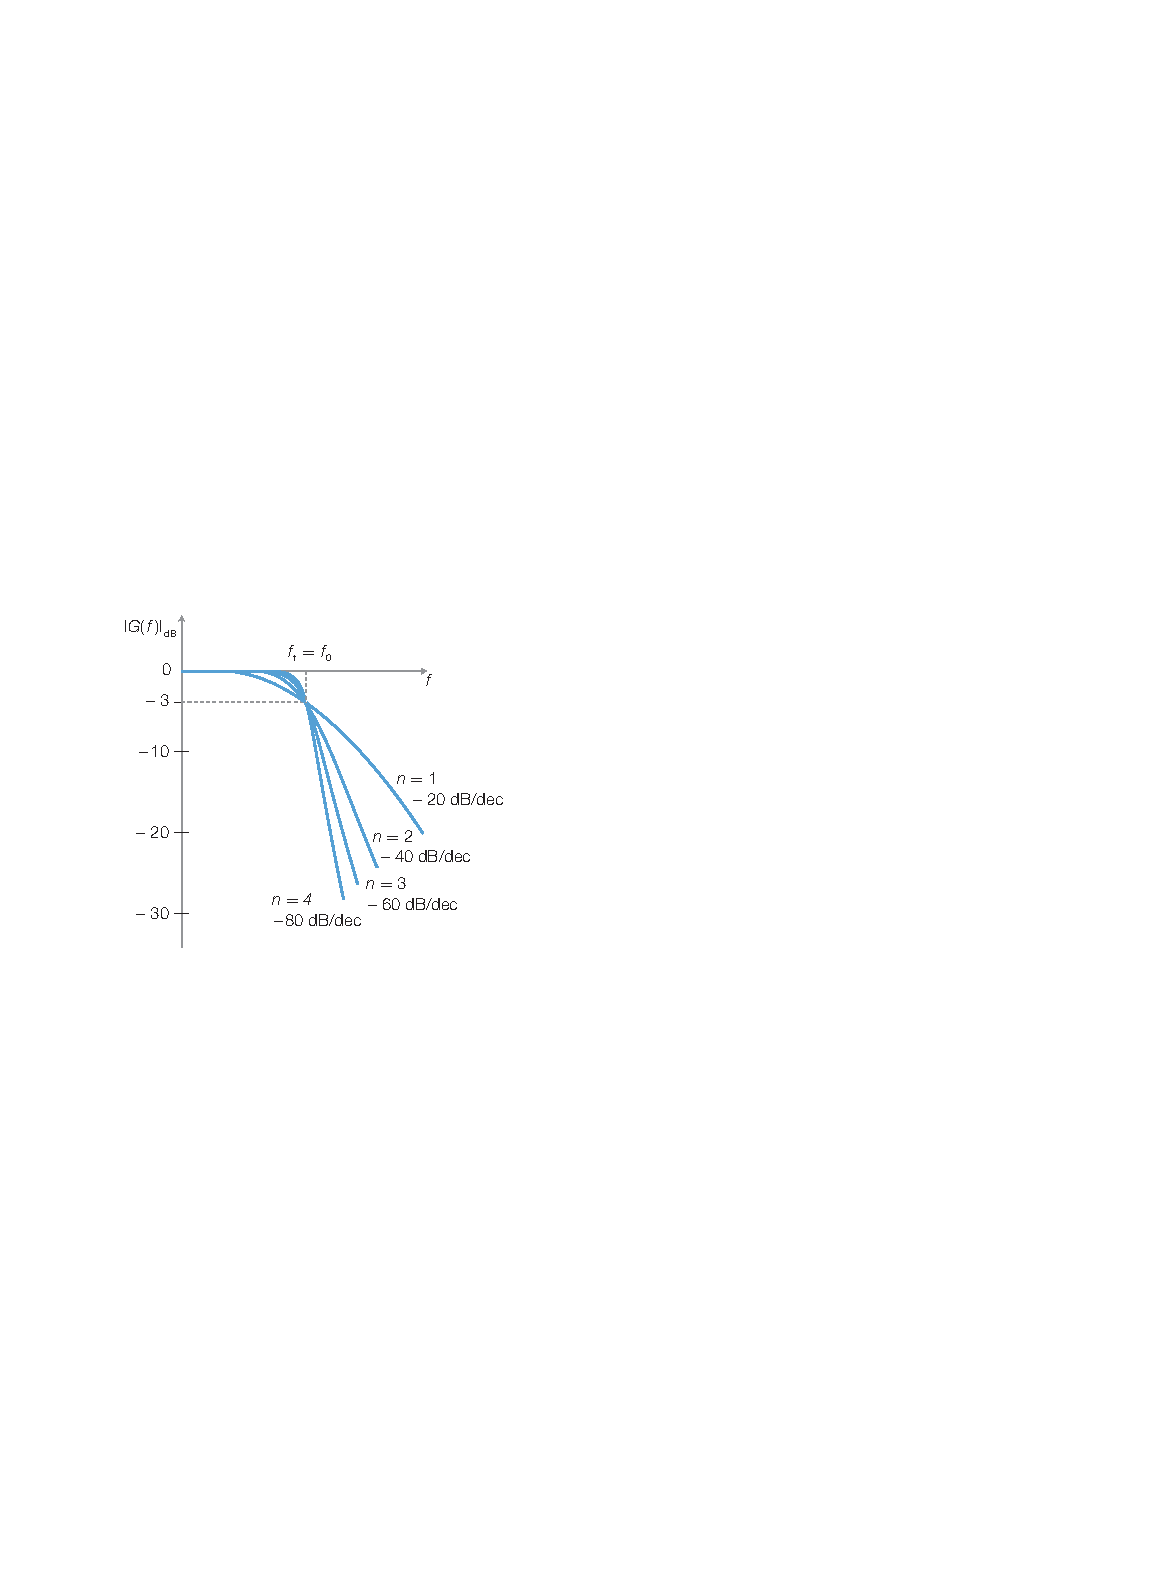
\includegraphics[width=.65\linewidth]{img/butterworth_ordini_vettoriale.pdf}
    \caption{Differenza nell'andamento del grafico di un filtro passa-bassa Butterworth con l'aumento o la diminuzione dell'ordine. L'aumento
        o la diminuzione della pulsazione di taglio sposta, rispettivamente, a destra o sinistra l'inizio della discesa \cite{mirandola_2012_progettazione}.
    }
    \label{fig:grafico_Butterworth}
\end{figure}

Per poter creare usando Python un filtro di quest tipo si usa la funzione:

\( \texttt{signal.butter(ordine, freq\_taglio\_norm, 'low', output='sos')} \).

\begin{equation}
    f_\text{norm}=\frac{2 f_s}{f_c}
    \label{eq:frequenza_taglio_normalizzata}
\end{equation}
L'argomento \texttt{frequenza\_taglio\_normalizzata} indica la frequenza di taglio normalizzata, definita nell'\autoref*{eq:frequenza_taglio_normalizzata}
dove $f_s$ è la frequenza di taglio effettiva e $f_c$ è la frequenza di campionamento, che si ricava facendo l'inverso della differenza di
due istanti di tempo consecutivi presenti nel dataset e che, in questo caso, risulta essere \SI{2}{\giga\hertz}.

Per stabilire il valore della $f_s$ si può osservare dal grafico della \autoref*{fig:20240502_single_bias_42V_trig_m50mV_box_indoor} che
l'intervallo di tempo che passa dal momento in cui la tensione iniza a diminuire a quello in cui ritorna al valore iniziale è di circa
\SI{1}{\micro\second}. Questo è l'intervallo di tempo che il SiPM impiega per ritornare nello stato di attesa del fotone, per questo motivo è
lecito tagliare tutte le frequenze maggiori di questa, cioè tutte le frequenze $>\SI{1}{\mega\hertz}$. Dall'~\autoref*{eq:frequenza_taglio_normalizzata}
si ricava l'\autoref*{eq:valore_f_norm}.
\begin{equation}
    f_\text{norm}=\frac{2 f_s}{f_c}=0.001
    \label{eq:valore_f_norm}
\end{equation}

Nel caso preso in esame si è scelto un filtro di ordine $n=1$. Il grafico del segnale filtrato è riportato nella \autoref*{fig:20240502_single_bias_42V_trig_m50mV_box_indoor__filtrato}.
La ragione per la quale è stato scelto un filtro di ordine 1 è che questo ordine garantisce la maggiore fedeltà all'andamento del grafico
non filtrato.
\begin{figure}[h!]
    \centering
    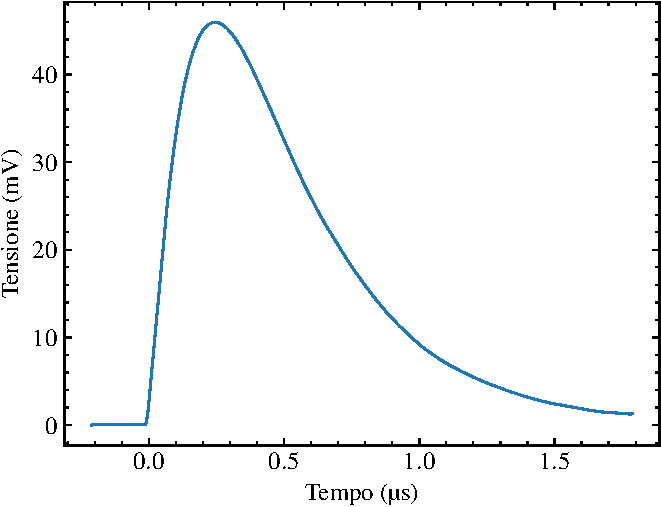
\includegraphics[width=.75\linewidth]{img/20240502_single_bias_42V_trig_m50mV_box_indoor__filtrato.pdf}
    \caption{Grafico ottenuto a partire dall'applicazione di un filtro passa-basso di Butterworth al grafico della \autoref*{fig:20240502_single_bias_42V_trig_m50mV_box_indoor}.}
    \label{fig:20240502_single_bias_42V_trig_m50mV_box_indoor__filtrato}
\end{figure}

Per avere un numero di dati apprezzabile, è stata effettuata un'acquisizione con una durata complessiva di 30 minuti e un trigger di
\SI{10}{\milli\volt} al fine di garantire un numero di eventi sufficientemente alto da avere una statistica sufficientemente comparabile
alla stima iniziale di 1 muone per \si{\square \centi \meter} per minuto. Avendo uno scintillatore con una area di rivelazione di 
\SI{150}{\square \centi \meter} si stima un numero di eventi pari a 4500. Tuttavia, considerando che il modello BC-422 usato ha un'efficienza
del 55\% e delle problematiche che possono insoregere a causa dell'output, è ragionevole prevedere un numero di misure che si attesti 
intorno alla metà del valore teorico. Avendo organizzato la lettura del segnale del SiPM con il connettore a T, il segnale viene acquisito 
dall'oscilloscopio quando uno dei due SiPM rivelava il passaggio del muone. Se durante la finestra di tempo che l'oscilloscopio occupa
per rivelare e salvare i dati arrivasse un altro muone, questo non verrebbe rivelato dall'oscilloscopio. Allo stesso modo, se un altro
muone colpisse lo scintillatore nel momento in cui il SiPM sta tornando in attesa, questo non verrebbe rivelato. Entrambe le situazioni descritte
portano ad una diminuzione delle misure. A partire da queste considerazioni, il numero di 2164 acquisizioni ottenute in 30 minuti
risulta del tutto in linea con quanto atteso.

Ogni muone incidente sullo scintillatore ha un'energia diversa che porta ad avere un numero di fotoni rilasciati dallo scinitllatore 
dipendente dall'angolo di incidenza che il muone ha rispetto alla superficie dello scintillatore.
Il numero di fotoni rilasciati dallo scintillatore fa generare dal SiPM risposte temporali con valori di picco di ampiezza diversa.
Risulta quindi di notevole interesse analizzare l'andamento della distribuzione delle tensioni di picco e, per fare ciò,, è sufficiente calcolare il valore massimo
ottenuto in ogni misura e creare poi un istogramma. Si ottiene così il grafico della \autoref*{fig:istogramma_minimi}.
\begin{figure}[h!]
    \centering
    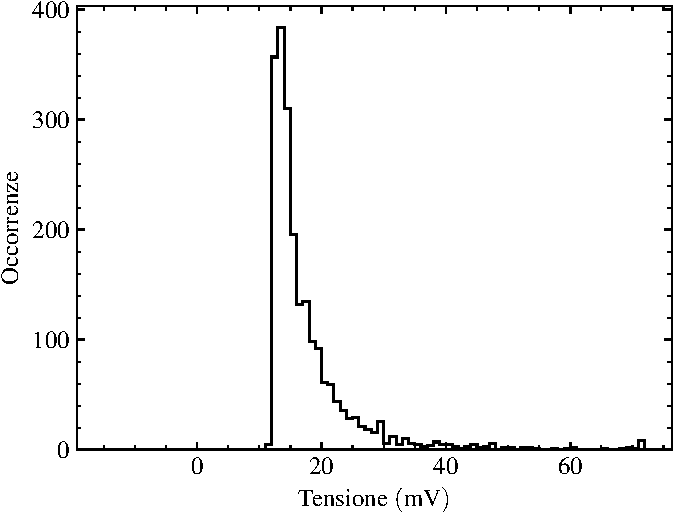
\includegraphics[width=.75\linewidth]{img/istogramma_minimi.pdf}
    \caption{Istrogramma dei valori minimi delle misure}
    \label{fig:istogramma_minimi}
\end{figure}

È stato dimostrato che i depositi di energia delle particelle su un materiale seguono una distribuzione detta di Landau. Questa distribuzione
ha un'equazione per calcolare la probabilità di un determinato evento estremamente complessa, che può essere approssimata usando l'\autoref*{eq:landau_semplificata}:
\begin{equation}
    p(x) = e^{-\frac{1}{2} \frac{x - \mu}{c} + e^{-\frac{x - \mu}{c}}}
    \label{eq:landau_semplificata}
\end{equation}
Nell'\autoref*{eq:landau_semplificata}, il simbolo $\mu$ è una costante di traslazione che sposta a destra o sinistra il grafico, mentre il 
simbolo $c$ è un parametro di scala che aumenta o diminuisce l'ampiezza della curva \.
Graficamente appare come si vede dall'immagine \autoref*{fig:Landau_Distribution_PDF}. 
In questo tipo di distribuzione non esiste un modo per calcolare media e varianza analiticamente, ma possono essere usati dei valori associabili,
ricavati attraverso passaggi empirici lavorando direttamente sul grafico. In questo caso la media corrisponderà al valore più probabile ($MPV$), cioè al valore di picco del grafico, 
mentre la deviazione standard, che verrà indicata con $\sigma$, viene definita come la differenza di ascisse tra i punti a ordinata pari a metà
del picco.
\begin{figure}[h!]
    \centering
    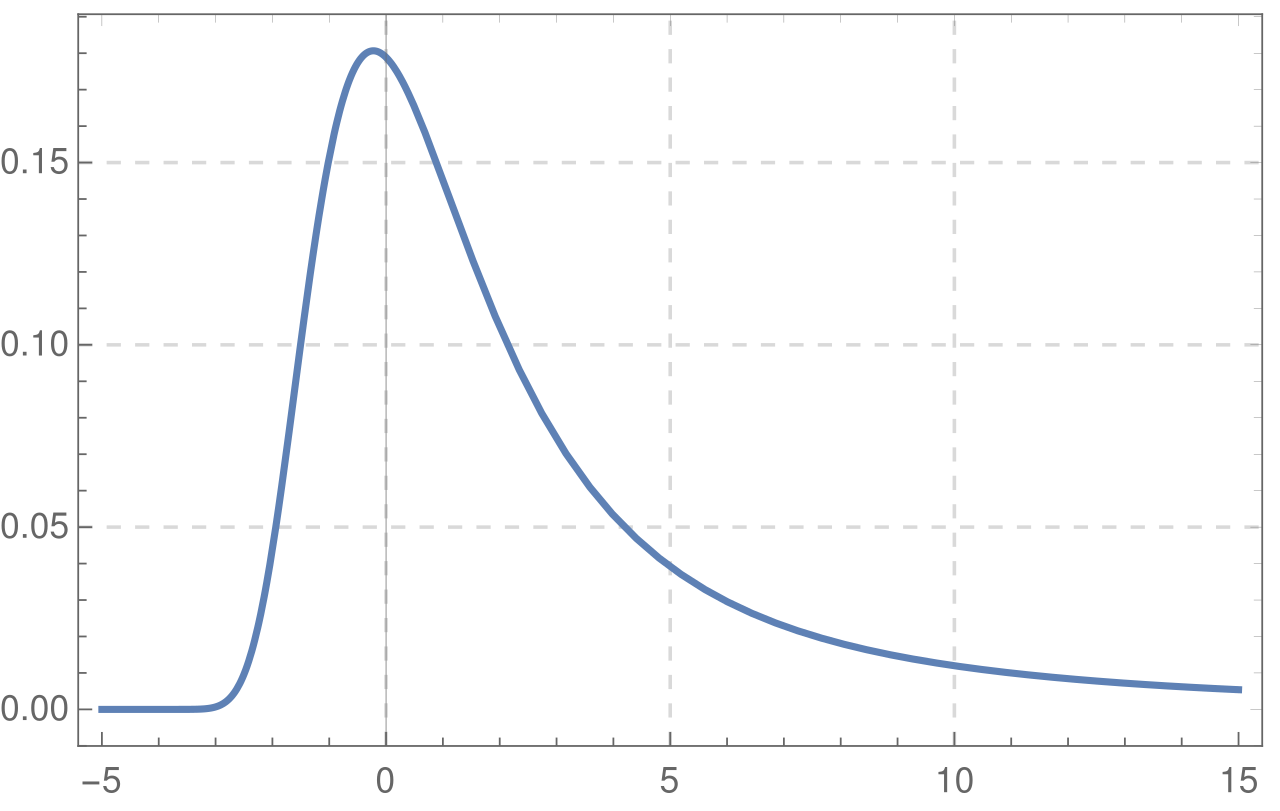
\includegraphics[width=.75\linewidth]{img/Landau_Distribution_PDF.svg.png}
    \caption{Andamento della distribuzione di Landau}
    \label{fig:Landau_Distribution_PDF}
\end{figure}

Ci aspettiamo quindi che anche le nostre misure seguano l'andamento della Landau, dobbiamo disegnare quindi una funzione che includa 
la maggior parte dei valori presenti nell'istogramma. La funzione più fedele è quella mostrata nel grafico della \autoref*{fig:muons_landau_fit}.
Si può notare che per alcuni valori dell'istogramma non collimano esattamente gli esatti corrispondenti nella distribuzione. Questo può
essere dovuto ad un numero di eventi non abbastanza alto, però, soprattutto per i valori maggiori, la funzione si adatta molto bene all'andamento
prodotti dall'istogramma.
\begin{figure}[h!]
    \centering
    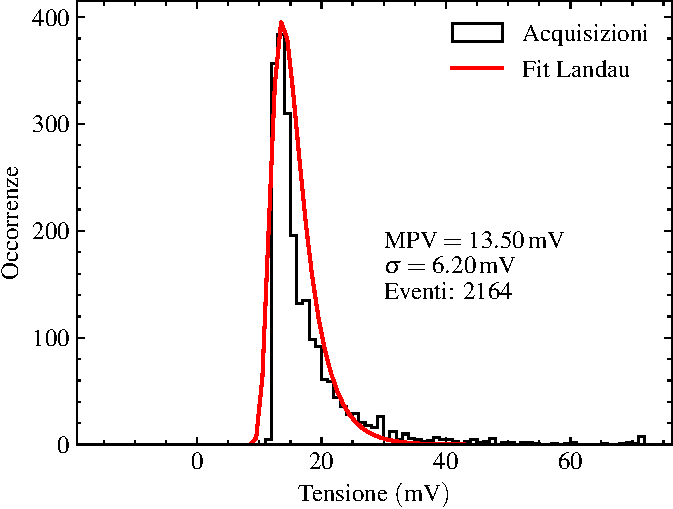
\includegraphics[width=.75\linewidth]{img/muons_landau_fit.pdf}
    \caption{Fit della distribuzione di Landau sui valori ottenuti dall'istogramma.}
    \label{fig:muons_landau_fit}
\end{figure}

Si è detto che questo tipo di misure possono portare al salvataggio di rivelazione errate che vengono attivate da un passaggio della tensione
al valore di trigger. Per eliminare eventuali misure rumorose che possono generarsi, si deve prima stabilire quando una rivelazione va 
considerata rumorosa. Nel caso di studio presentato, si considera una misura rumorosa se non rispetta l'andamento della
\autoref*{fig:20240502_single_bias_42V_trig_m50mV_box_indoor__filtrato}.
Un'osservazione che si può fare riguardo all'andamento del grafico è che il suo valore medio è compreso tra il picco della curva e il momento
in cui la curva si trova in stato di riposo. Osservando la \autoref*{fig:20240502_single_bias_42V_trig_m50mV_box_indoor__filtrato},
possiamo affermare che un grafico corretto attraversa il valore medio due volte. Tuttavia, anche se il grafico è filtrato, non si può
stabilire con certezza che questo attraversi il valore medio due volte dato che potrebbero esserci comunque delle minime oscillazioni.
Una possibile soluzione a questo problema è andare a calcolare la media degli attraversamenti del valor medio di ogni grafico e
considerare rumorosi i grafici con un numero di attraversamenti di molto superiore alla media, per esempio il doppio.
Agendo in questo modo vengono scartate 36 acquisizioni, di cui si vedono due esempi significativi nella \autoref*{fig:scarti}.

\begin{figure}[h!]
    \centering
    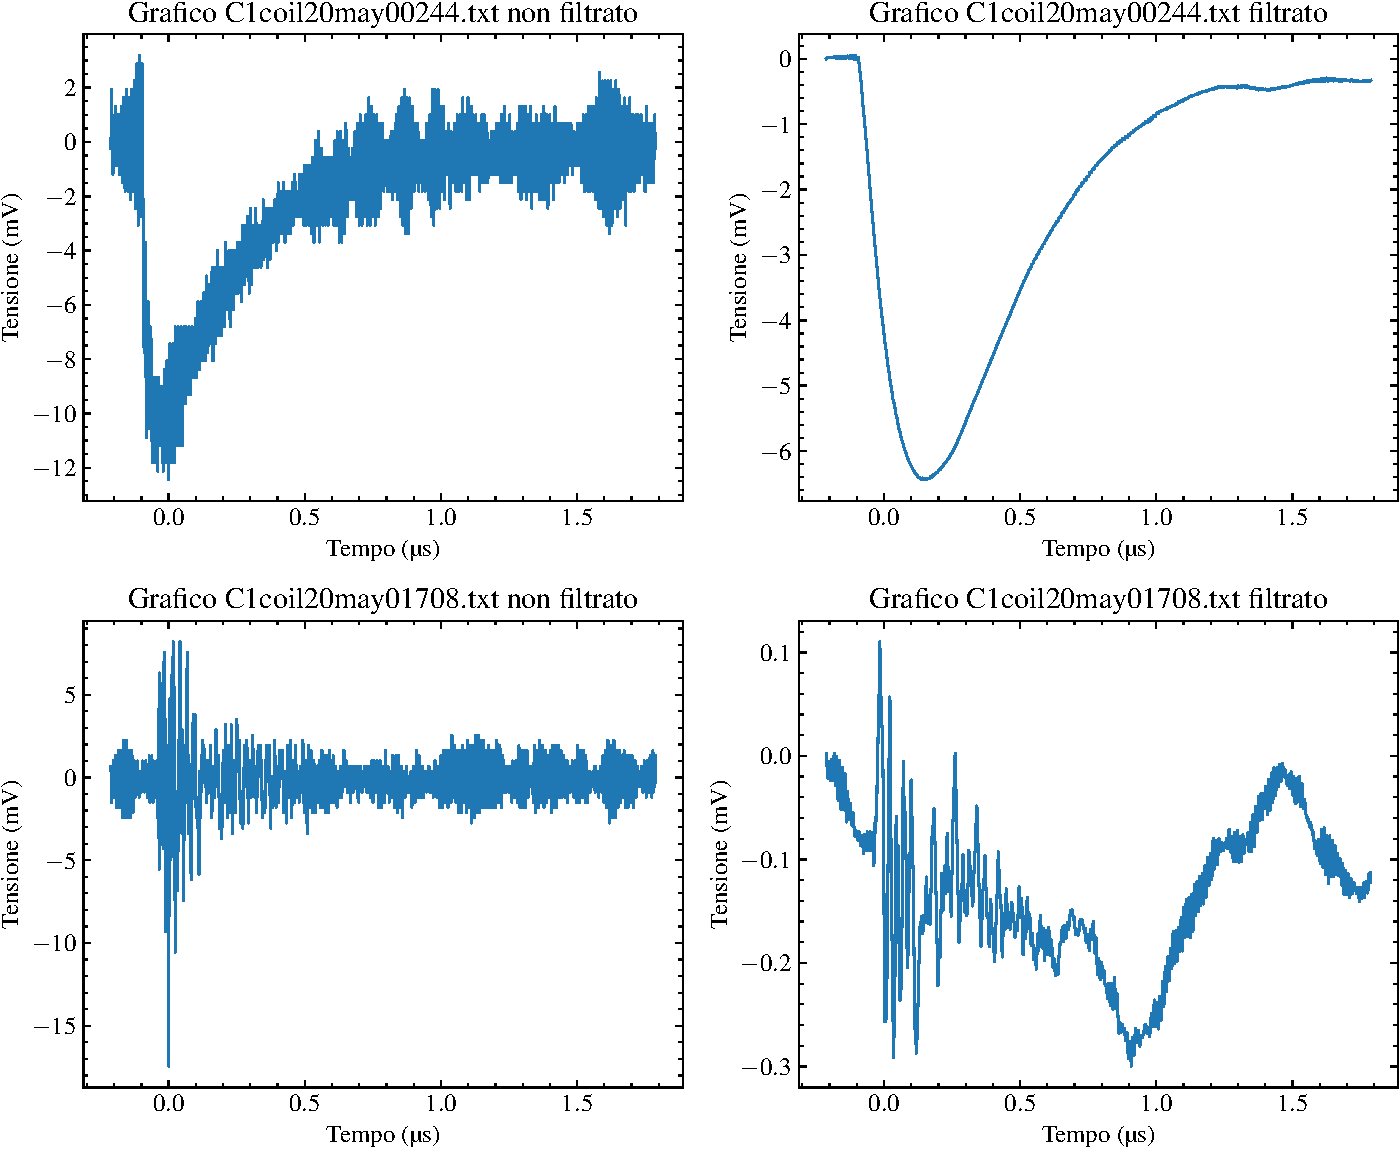
\includegraphics[width=.85\linewidth]{img/scarti.pdf}
    \caption{Due esempi di grafici scartati in cui vengono riportati la versione non filtrata e quella filtrata}
    \label{fig:scarti}
\end{figure}

Osservando il grafico "C1coil20may00244" questo presenta in realtà un andamento simile al riferimento,
tuttavia osservando la parte crescente del grafico non filtrato si notano una serie di oscillazioni poco ampie
che influiscono nella valutazione e che continuano ad essere presenti a causa della loro ampiezza nel grafico non filtrato. Quindi,
considerando anche il loro numero a confronto del totale dei grafici ottenuti, si può ritenere che anche se questi vengono scartati il risultato
dell'analisi è pur sempre verosimile. Osserando, invece, l'andamento del garfico "C1coil20may01708", si può ritenere che questi siano effettivamente
misurati a seguito di un rumore esterno, probabilmente ua certa quantità di luce esterna che ha colpito il SiPM.
Avendo scartato solo 36 misure su 2164 si può affermare che il setup preparato è molto preciso e affidabile e si può prevedere che, rifacendo
l'istogramma dell'andamento dei valori minimi come quello della \autoref*{fig:istogramma_minimi} i valori di $MPV$ e $\sigma$ non cambieranno molto.
Come si può vedere dalla \autoref*{fig:istogramma_minimi_selezionati}; l'$MPV$ rimane lo stesso. Nel secondo caso, invece, $\sigma$ 
diminuisce di \SI{2,63}{\milli\volt}, cioè dell'$53,84\%$ rispetto alla media dei due $\sigma$.

\begin{figure}[h!]
    \centering
    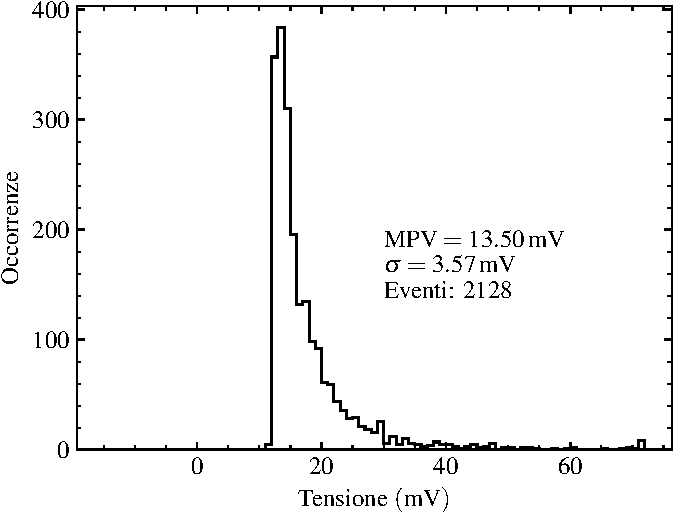
\includegraphics[width=.85\linewidth]{img/istogramma_minimi_selezionati.pdf}
    \caption{Istogramma della distribuzione dei depositi di energia dei muoni con escluse le misure rumorose.}
    \label{fig:istogramma_minimi_selezionati}
\end{figure}

In conclusione, in questo capitolo è stato spiegato come realizzare un sistema in grado di rivelare l'arrivo dei muoni sulla superficie
terrestre e è stato mostrato un esempio di come poter analizzare i dati ottenuti secondo le proprie esigenze usando anche una distribuzione
statistica propria di questo tipo di problema come la distribuzione di Landau. I dati elaborati dal procedimento
descritto in questa parte possono anche essere condivisi tra diverse unità di raccolta dati, come previsto dal progetto MuonPi.
